\documentclass[12pt,a4paper]{article}
\usepackage{ctex}
\usepackage{amsmath,amscd,amsbsy,amssymb,latexsym,url,bm,amsthm}
\usepackage{epsfig,graphicx,subfigure}
\usepackage{enumitem,balance}
\usepackage{wrapfig}
\usepackage{mathrsfs,euscript}
\usepackage[usenames]{xcolor}
\usepackage{hyperref}
\usepackage[vlined,ruled,linesnumbered]{algorithm2e}
\usepackage{array}
\usepackage{float}
\hypersetup{colorlinks=true,linkcolor=black}

\newtheorem{theorem}{Theorem}
\newtheorem{lemma}[theorem]{Lemma}
\newtheorem{proposition}[theorem]{Proposition}
\newtheorem{corollary}[theorem]{Corollary}
\newtheorem{exercise}{Exercise}
\newtheorem*{solution}{Solution}
\newtheorem{definition}{Definition}
\theoremstyle{definition}

\renewcommand{\thefootnote}{\fnsymbol{footnote}}

\newcommand{\postscript}[2]
 {\setlength{\epsfxsize}{#2\hsize}
  \centerline{\epsfbox{#1}}}

\renewcommand{\baselinestretch}{1.0}

\setlength{\oddsidemargin}{-0.365in}
\setlength{\evensidemargin}{-0.365in}
\setlength{\topmargin}{-0.3in}
\setlength{\headheight}{0in}
\setlength{\headsep}{0in}
\setlength{\textheight}{10.1in}
\setlength{\textwidth}{7in}
\makeatletter \renewenvironment{proof}[1][Proof] {\par\pushQED{\qed}\normalfont\topsep6\p@\@plus6\p@\relax\trivlist\item[\hskip\labelsep\bfseries#1\@addpunct{.}]\ignorespaces}{\popQED\endtrivlist\@endpefalse} \makeatother
\makeatletter
\renewenvironment{solution}[1][Solution] {\par\pushQED{\qed}\normalfont\topsep6\p@\@plus6\p@\relax\trivlist\item[\hskip\labelsep\bfseries#1\@addpunct{.}]\ignorespaces}{\popQED\endtrivlist\@endpefalse} \makeatother

\begin{document}
\noindent

%========================================================================
\noindent\framebox[\linewidth]{\shortstack[c]{
\Large{\textbf{Lab07-Amortized Analysis}}\vspace{1mm}\\
CS214-Algorithm and Complexity, Xiaofeng Gao \& Lei Wang, Spring 2021.}}
\begin{center}
\footnotesize{\color{red}$*$ If there is any problem, please contact TA Yihao Xie. }

\footnotesize{\color{blue}$*$ Name:Yanjie Ze  \quad Student ID:519021910706\quad Email: zeyanjie@sjtu.edu.cn}
\end{center}
\begin{enumerate}
	\item Suppose we perform a sequence of n operations on a data structure in which the $i$ th 		operation costs $i$ if $i$ is an exact power of 2, and 1 otherwise. Use an accounting method to determine the amortized cost per operation.
\begin{solution}
Denote $C_i$ as the cost of the $i$th operation, then we will $C_i$'s formula:
    $$ 
			C_i=\left\{
            \begin{aligned}
            &i, &if\ i\ is\ the\ power\ of\ 2\\
            &1, &otherwise 
            \end{aligned}
            \right.
            $$
We can view this problem as a $Table\ Insert$ problem, and the formula can be explained as such:
\begin{itemize}
    \item If inserting the $i$th element doesn't lead to the full table, insert the element. The cost is $1$.
    \item If inserting the $i$th element leads to the full table, we should first expand the table and second copy all the old elements and also insert the new element. The cost is $i$.
\end{itemize}
For example, Fig~\ref{p1} illustrates the process of $insert(4)$. When we try to insert the $4$th element, we find that the table will be full after the insertion. So we first expand the table, and then copy and insert. The number in each box shows the cost, and the cost of $insert(4)$ is $4$, which consists of $3$ copys and $1$ insertion. 

\begin{figure}[H]
    \centering
    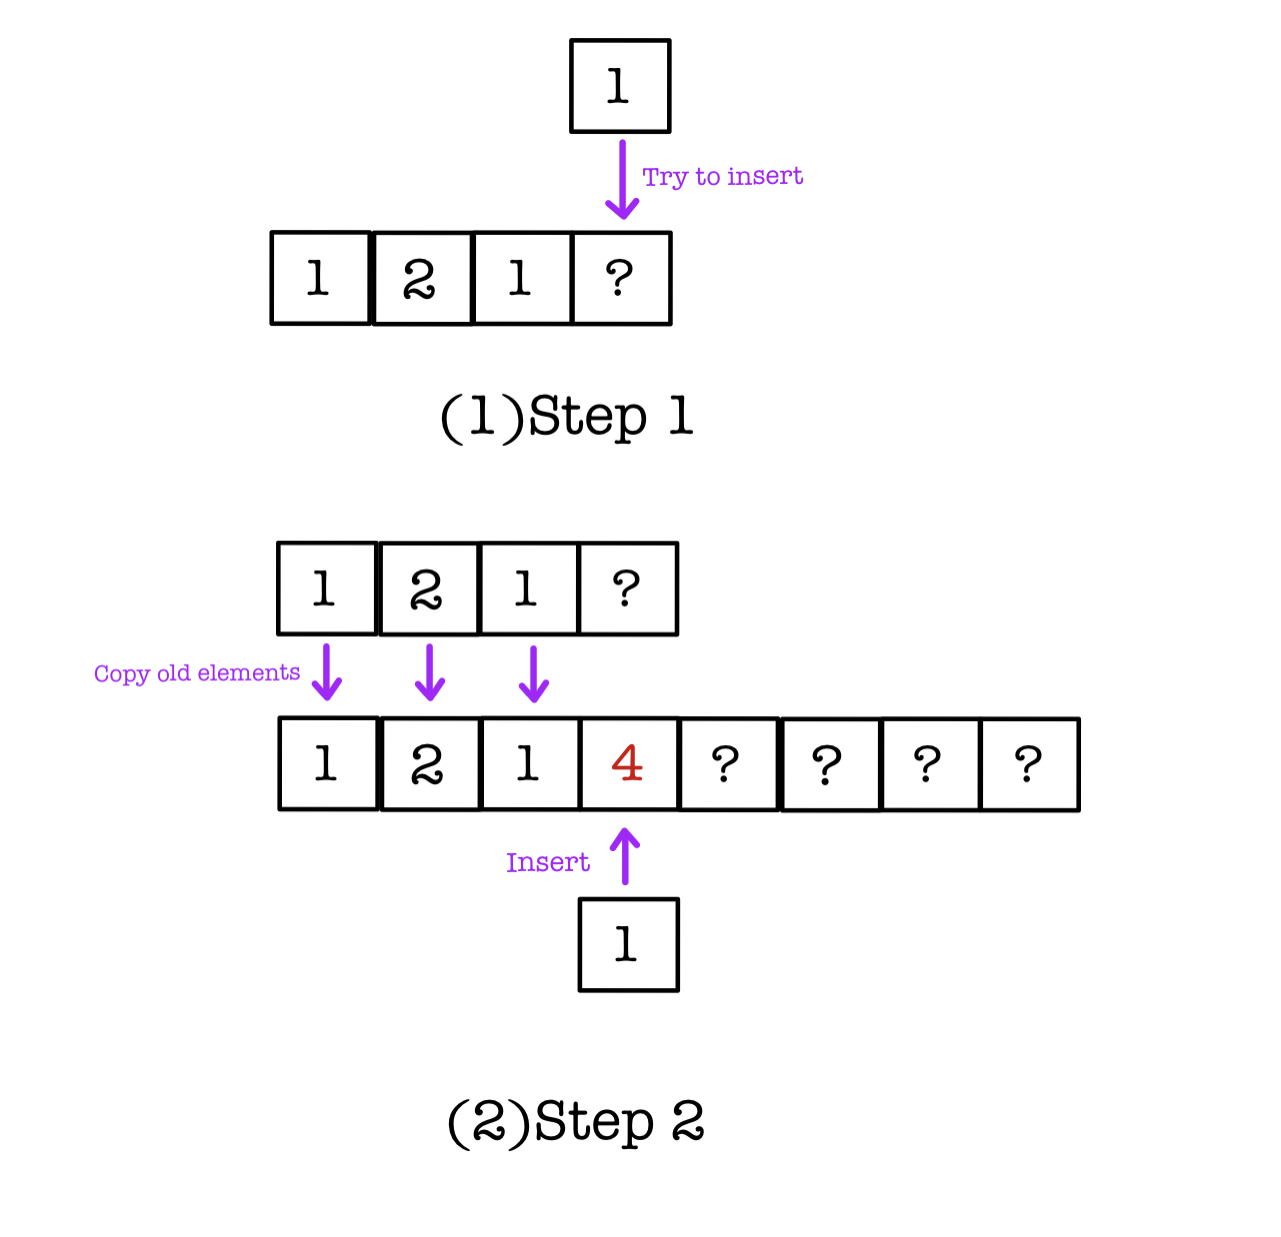
\includegraphics[width=10cm]{1.jpeg}
    \caption{Insert(4)}
    \label{p1}
\end{figure}

Therefore, for the $i$th operation, an amortized cost $\hat{C_i}=3\$$ is charged.
\begin{itemize}
    \item $1\$$ pays for the insertion itself.
    \item $1\$$ pays for the next copy of itself.
    \item $1\$$ pays for the next copy of an old element.
\end{itemize}

Denote $T(n)$ as the total cost of n operation, we have an upper bound by this \textbf{accounting method}:
$$
T(n) = \sum_{i=1}^n C_i \leq \sum_{i=1}^n \hat{C_i} = 3n
$$
And the amortized cost per operation is $3$.
\end{solution}
	\item Consider an ordinary \textbf{binary min-heap} data structure with $n$ elements supporting
the instructions \textsc{Insert} and \textsc{Extract-Min} in $O(\log n)$ worst-case time. Give a
potential function $\Phi$ such that the amortized cost of \textsc{Insert} is $O(\log n)$ and the
amortized cost of \textsc{Extract-Min} is $O(1)$, and show that it works.

\begin{solution}
~\\
\textbf{Potential Function}: 

Define state $S_i$ as the number of elements in the heap. Define the potential function $\Phi(S_i)$:
\begin{itemize}
    \item \textsc{Insert}:\quad $
\Phi(S_i)- \Phi(S_{i-1})= \log S_i
$
\item \textsc{Extract-Min}: \quad $
\Phi(S_i)- \Phi(S_{i-1})= -\log S_i
$
\end{itemize}
\textbf{Explanation}: 

When performing \textsc{Insert}, the heap will have more elements, which is viewed as the increase of potential energy and its height is also possible to rise. And the potential energy's quantity rests on the current height, which is similar to climbing: the higher position we are in, the more potential energy we have.

When performing \textsc{Extract-Min}, the heap's top element is extracted, and the heap needs to be adjusted. The action of adjustment will consume the potential energy accumulated before.

\textbf{Correctness}: 

Because \textsc{Extract-Min} will not perform when the heap has no elements, which means:
$$\Phi(S_i) \geq 0 = \Phi(S_0)$$
\textbf{Amortized Analysis}:
\begin{itemize}
\item $0 \leq S_i \leq n $
    \item \textsc{Insert}:\quad $
\hat{C_i} = C_i + \Phi(S_i) - \Phi(S_{i-1}) = 2\log S_i = O(\log n)
$
\item \textsc{Extract-Min}:\quad $
\hat{C_i} = C_i + \Phi(S_i)-\Phi(S_{i-1}) = 0 = O(1)
$
\end{itemize}

\end{solution}
	
	\item Assume we have a set of arrays $A_0, A_1, A_2,\cdots$, where the $i^{th}$ array $A_i$ has a length of $2^i$. Whenever an element is inserted into the arrays, we always intend to insert it into $A_0$. If $A_0$ is full then we pop the element in $A_0$ off and insert it with the new element into $A_{1}$. (Thus, if $A_{i}$ is already full, we recursively pop all its members off and insert them with the elements popped from $A_0,...,A_{i-1}$ and the new element into $A_{i+1}$ until we find an empty array to store the elements.) An illustrative example is shown in Figure \ref{Fig-MultiArray}. Inserting or popping an element take $O(1)$ time.

	\begin{figure}[!htbp]
	\centering
	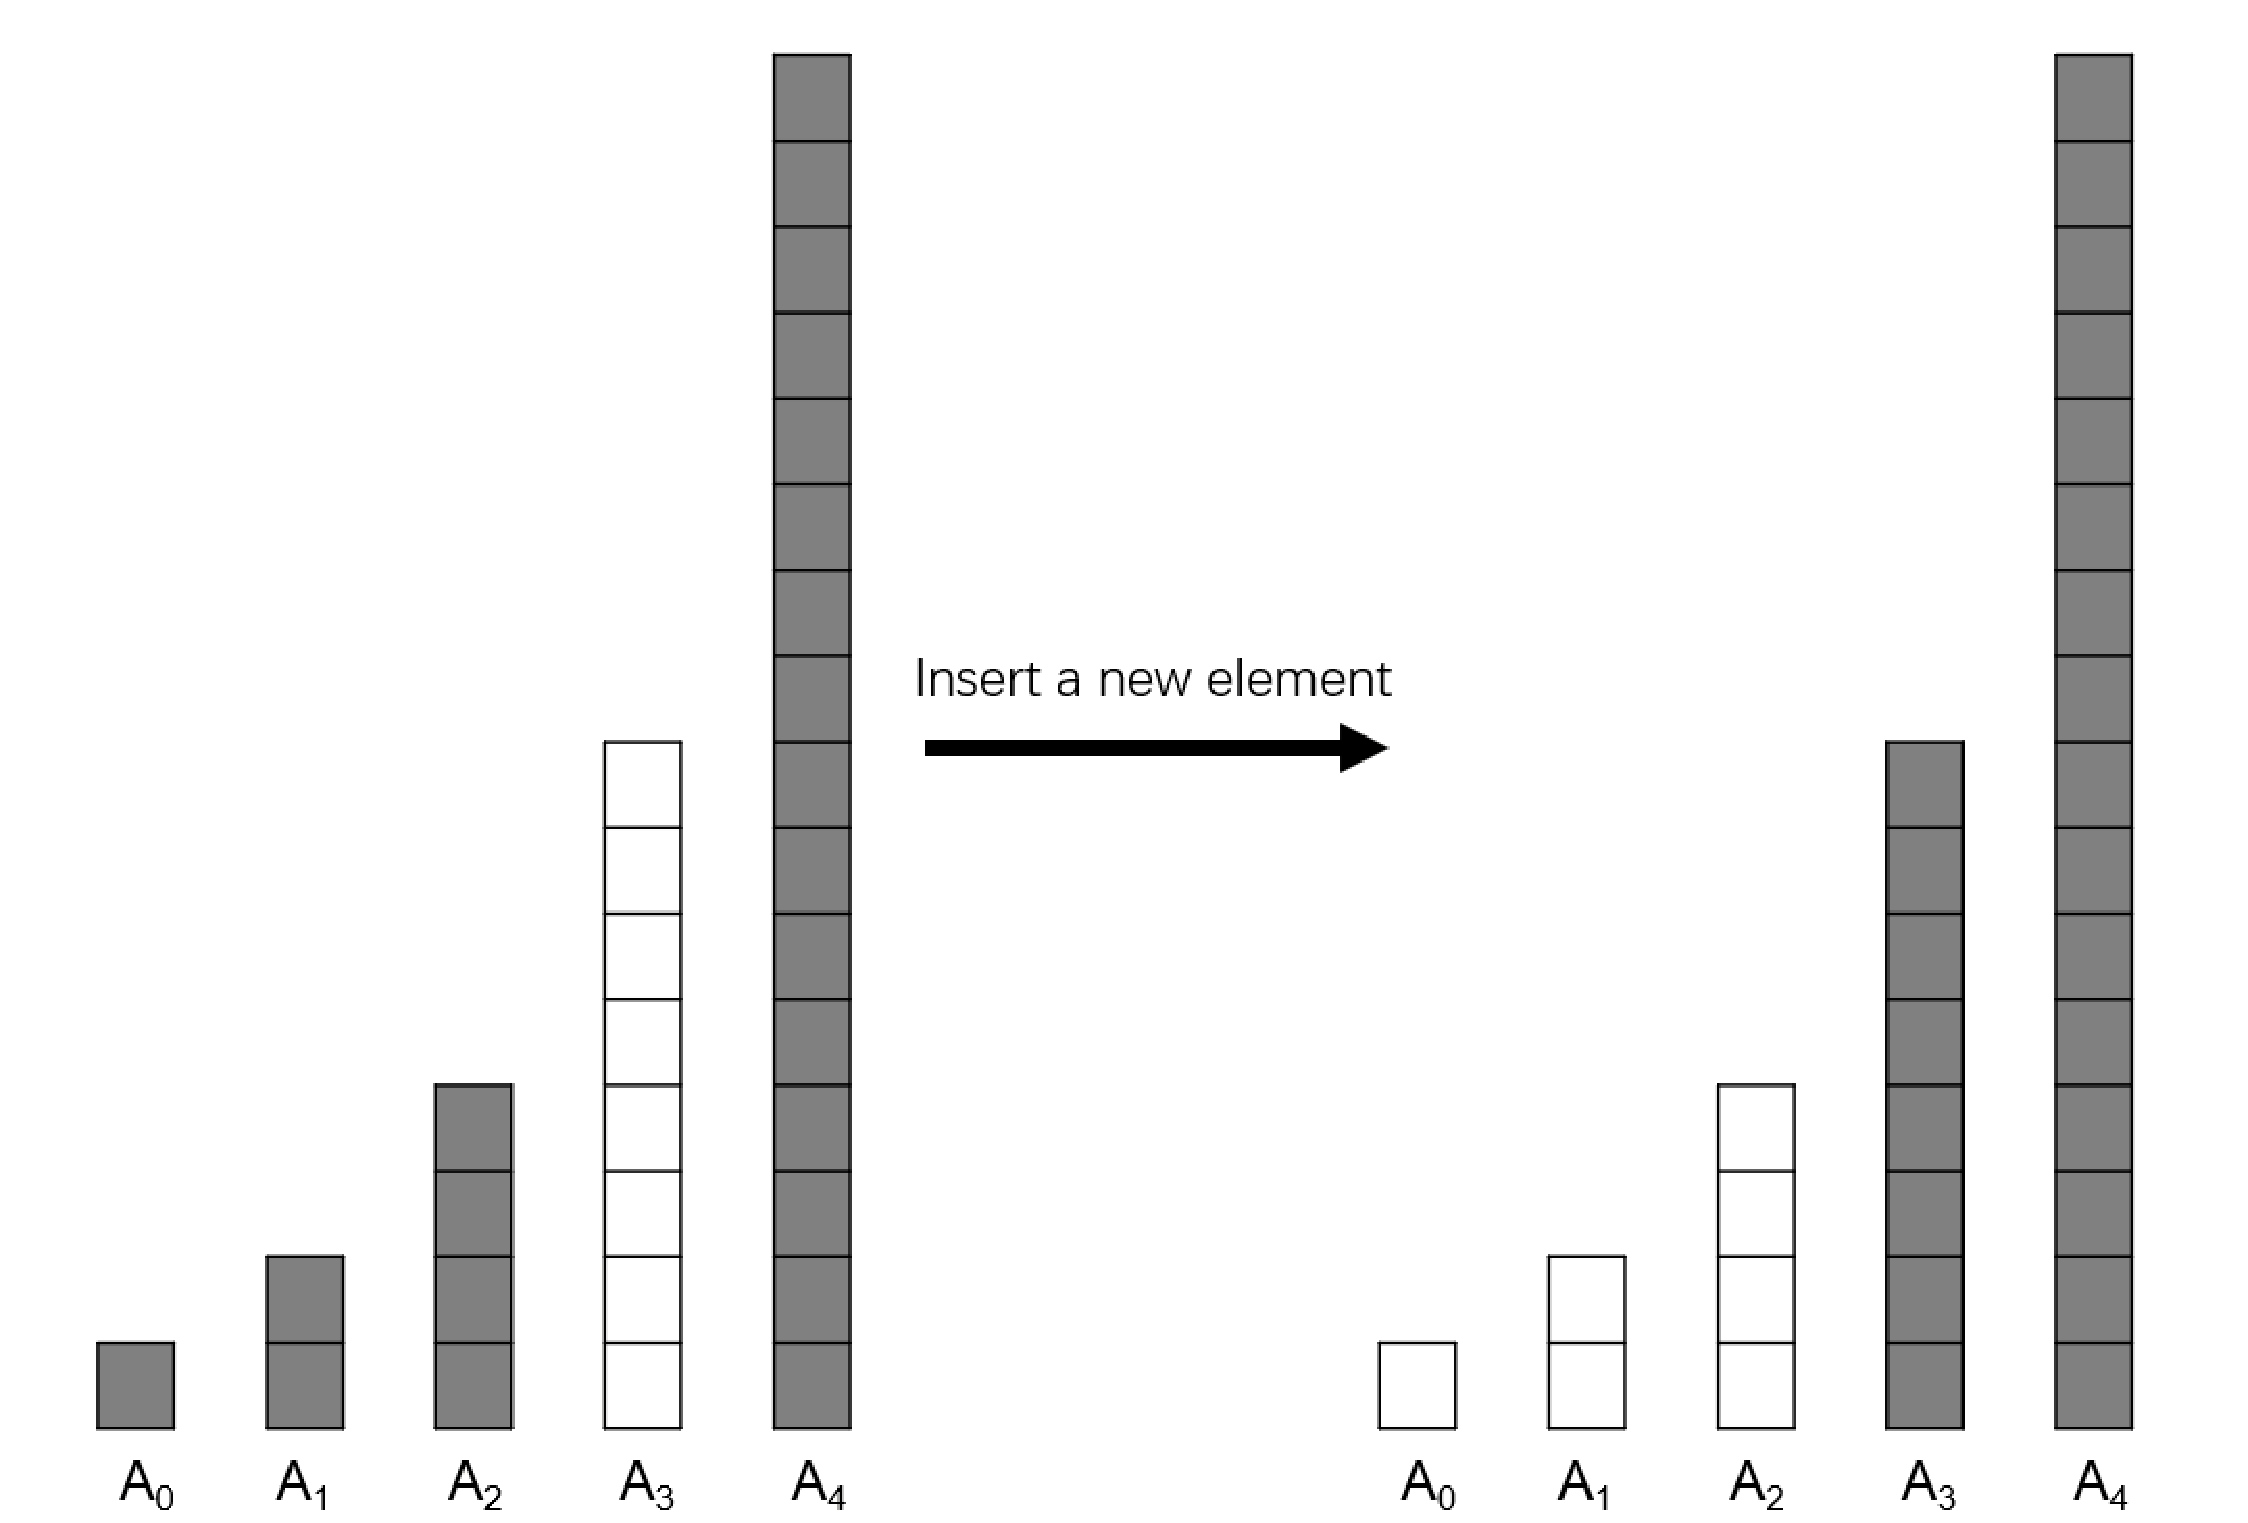
\includegraphics[width=0.5\textwidth]{Fig-MultiArray.pdf}
	\caption{An example of making room for one new element in the set of arrays.}
	\label{Fig-MultiArray}
	\end{figure}

    \begin{enumerate}
        \item In the worst case, how long does it take to add a new element into the set of arrays containing $n$ elements?
        \begin{solution}
        ~\\
        \textbf{Lemma 1}:\textit{If there exist elements in array $A_i$, array $A_i$ must be full, with $2^i$ elements.}
        
        \begin{proof}
        \textbf{Lemma 1} is naturally induced from the problem setting.
        
        For array $A_0,A_1,...,A_n$, they can store $\sum_{i=0}^n 2^i = 2^{n+1}-1$ elements.
        
        If $A_0,...,A_n$ are all full, inserting a new element will make all old elements and the new element into array $A_{n+1}$, which can exactly hold $2^{n+1}$ elements. Then, $A_{n+1}$ is full and the former arrays are  totally empty.
        
        Since $n$ can be any positive integer value, ranging from $1$ to $\infty$, we prove \textbf{Lemma 1} is correct.
        \end{proof}
        
        As shown in Fig.~\ref{p31}, \textsc{Insert(3)} fills $A_0$ to the full and \textsc{Insert(4)} fills $A_2$ to the full and empties $A_0$ and $A_1$, verifying \textbf{Lemma 1}.
        \begin{figure}[H]
            \centering
            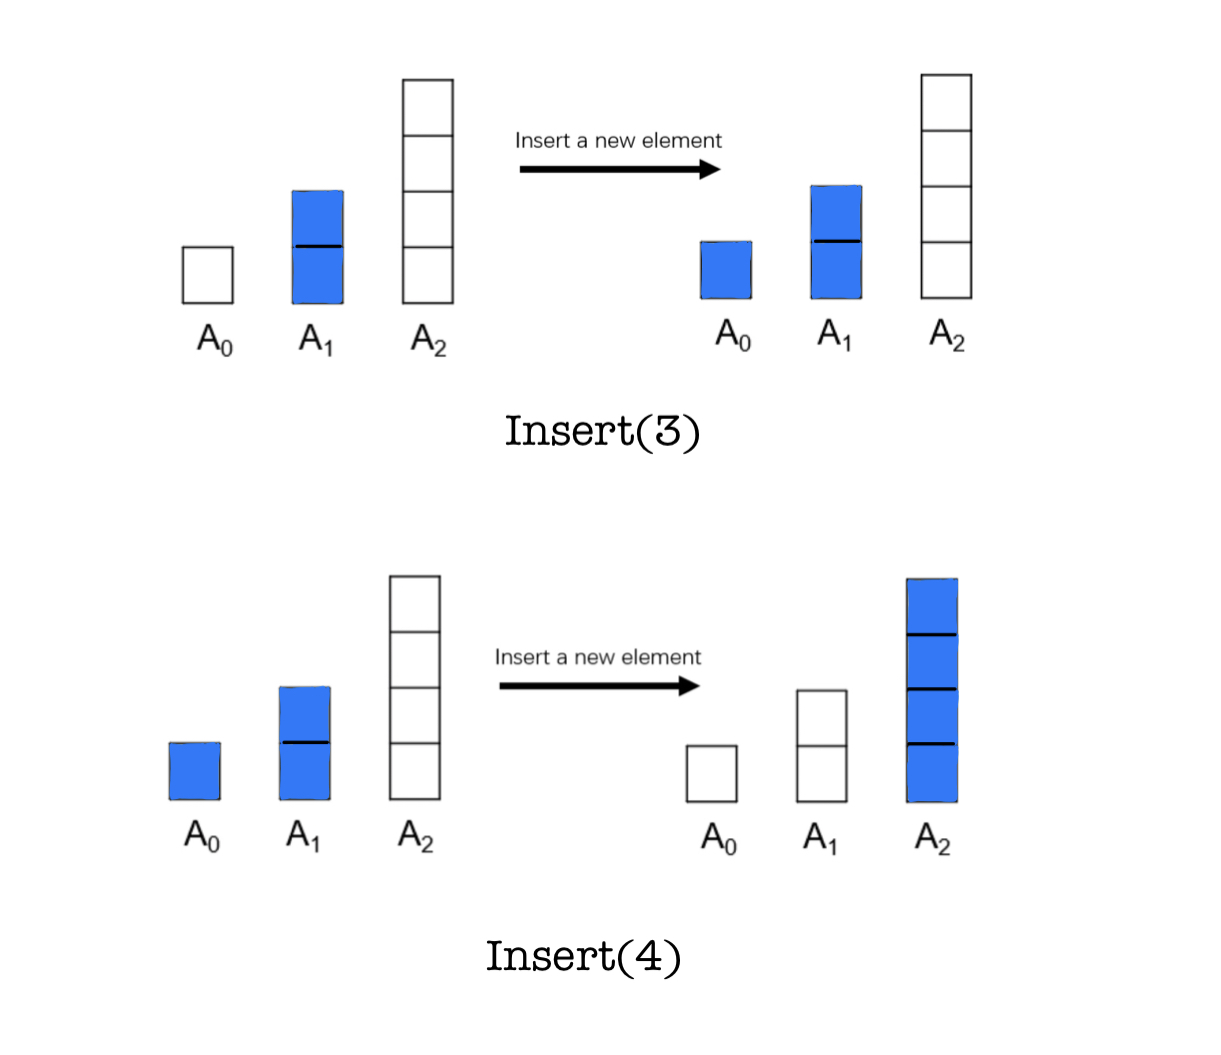
\includegraphics[width=10cm]{2.jpg}
            \caption{Process of Inserting}
            \label{p31}
        \end{figure}
        
        Based on \textbf{Lemma 1}, we know if there are $n$ elements in total, \textbf{the worst case} is that all elements are filled in $A_0, A_1,...,A_k$, with no middle empty arrays. In such case, $n=2^{k+1}-1, k =1,2,..$.
        
        The cost of \textsc{Insert(n+1)}is:
        $$
        cost_{worst} = n\times cost_{pop} + (n+1)\times cost_{push} = 2n+1 = O(n)
        $$
        \end{solution}
        
        \item Prove that the amortized cost of adding an element is $O(\log n)$ by \emph{Aggregation Analysis}.
        
        \begin{solution}
        ~\\
        First, we get the expression of $C_i$. 
        \begin{itemize}
            \item 
        When $i$ is odd, $C_i$ is equal to 1 obviously. 
        \item 
        When $i=2^k$, which is talked about in problem(a), $C_i=2n-1$. 
        \item
        When i isn't odd and is not equal to $i=2^k$, then $i$ must be an even number between $2^{k}$ and $2^{k+1}$, where $k=\lfloor \log_2 n\rfloor$. In this case, there exists one or more empty array in array $A_0, A_1,...,A_k$. So the pattern of the change of $C_i$ is similar to that before. For example, $C_1$ to $C_{32}$ is:
        \begin{center}
        
        1, {\color{red}3}, 1, {\color{red}7}, 1, 3, 1, {\color{red}15}\\
        1, 3, 1, 7, 1, 3, 1, {\color{red}31}\\
        1, 3, 1, 7, 1, 3, 1, 15\\
        1, 3, 1, 7, 1, 3, 1, {\color{red}63}\\
        
        \end{center}
        \end{itemize}
        Therefore, the expression of $C_i$ is :
        $$
        C_i = \left\{
        \begin{aligned}
        &1, &when\ i\ is\ odd.\\
        &2i-1, &when\ i=2^k,k\in \mathbb{N}\\
        &2(i-2 ^{\lfloor \log_2 i\rfloor})-1 ,&otherwise\\
        \end{aligned}
        \right.
        $$
        Thus,
        $$
        \begin{aligned}
        T(n)  
        &=\sum_{i=1}^n C_i\\
        &=\sum_{odd}1 + \sum_{k=1}^{\lfloor \log_2 n\rfloor}(2\times 2^k-1)+\sum_{otherwise}(2(i-2 ^{\lfloor \log_2 i\rfloor})-1)\\
        &\leq \frac n2 + 4(n-1)-\log_2n + \sum_{otherwise}(2(i-2 ^{\lfloor \log_2 i\rfloor})-1) \\
        &\leq \frac 92 n - \log_2 n + \sum_{k=1}^{\lfloor \log_2 n \rfloor+1} (2n-1)\\
        &=\frac 92 n - \log_2 n + (\lfloor \log_2 n \rfloor+1)(2n-1)\\
        & = O(n\log n)
        \end{aligned} 
        $$
        Finally, by \textbf{Aggregation Analysis},we get the amortized cost of adding an element is:
        $$
        \frac{T(n)}{n} = O(\log n)
        $$
        
        \end{solution}
        \item If each array $A_i$ is required to be sorted but elements in different arrays have no relationship with each other, how long does it take in the worst case to search an element in the arrays containing $n$ elements? 
        \begin{solution}
        The cost of searching an element in $A_i$ using \textbf{Binary Search} is $O(\log|A_i|)$.
        
        In the worst case, to search an element, we need to search it in all arrays.  What's more, there exists no empty array in $A_0, A_1,...,A_k,n=2^{k+1}-1$.
        
        This is because:
        $$
        \log|A_0| + \log|A_1| + ... + \log|A_k| = \log(|A_0|\times|A_1|...\times|A_k|)>\log|A_{k+1}|
        $$
        Which means searching elements distributed in different arrays takes more time.
        ~\\
        
        Thus, the total cost of searching an element is:
        $$
        \begin{aligned}
        cost_{worst} &= O(\log|A_0|) + O(\log|A_1|)+...+O(\log|A_k|)\\
        &=O(\log(|A_0|\times|A_1|...\times |A_k|))\\
        &=O(\log(2^{0+1+...+k})) \\
        &=O(\log(2^{\frac{k^2+k}{2}}))\\
        &=O(k^2)\\
        &=O(\log^2n)
        \end{aligned}
        $$
        \end{solution}
\item What is the amortized cost of adding an element in the case of (c) if the comparison between two elements also takes $O(1)$ time?
\begin{solution}
~\\
The cost of adding an element without comparison is shown in problem(b). For adding an element and making the array in order, the cost consists of three parts:\textbf{pop,sort,push}.
\begin{itemize}
    \item When $i$ is odd, $C_i$ is still 1.
    \item When $i=2^k$, there are $i-1$ elements in need of sorting after pop operation. \textbf{Quick Sort} costs $O(i\log i)$ in average.
    \item Otherwise, there are $m=i-2 ^{\lfloor \log_2 i\rfloor}$ elements in need of sorting after pop operation, costing $O(m\log m)$ in average.
\end{itemize}
Thus, we have the expression of $C_i$:
$$
        C_i = \left\{
        \begin{aligned}
        &1, &when\ i\ is\ odd.\\
        &2i-1+O(i\log i), &when\ i=2^k,k\in \mathbb{N}\\
        &2m-1+O(m\log m) ,where\ m=i-2 ^{\lfloor \log_2 i\rfloor}, &otherwise\\
        \end{aligned}
        \right.
        $$

Therefore, amortized cost is $O(\log^2n)$(I guess).
\end{solution}
    \end{enumerate}
	
\end{enumerate}



\textbf{Remark:} Please include your .pdf, .tex files for uploading with standard file names.


%========================================================================
\end{document}
